The first step when designing circuits is creating the schematic.
Since the design is mainly digital (theres only four analog signals), it 
can be easily cutted down into differents blocks.

We're going to dig into different parts of this process !

\section{Analog conception}
For the first part, let's discover the analog stuff we've done on the board.
The analog is quite absent on this board, and we only use it for two purposes :
\begin{itemize}
    \item   Get the position feedback of the servos
    \item   Monitor voltages on power rails
\end{itemize}

For the first part, we're measuring a DC voltage that move between $~0.6 \si{\volt}$
and $~2.4 \si{\volt}$. And, they're moving slowly, it take near one second to get
from one limit to the other !

Since the voltage is already in our measurement range, and even more, in the area
where the integrated ADC is quite linear, we don't have a lot of signal conditioning 
to do.

We've only designed a filter to remove any high frequency signals that may be picked
by the wires used. Thus, we designed a Sallen-Key active filter, with a 100 Hz cutoff
frequency.

The circuit is the following one :
\begin{figure}[!ht]
    \centering
    \resizebox{\SchematicWidth}{!}{%
        \begin{circuitikz}
            \tikzstyle{every node}=[font=\normalsize]
            \draw (5,12.25) to[european resistor,l={ \normalsize R1 = 16k$\Omega$}] (7.5,12.25);
            \draw (8.75,12.25) to[european resistor,l={ \normalsize R2 = 16k$\Omega$}] (11.25,12.25);
            \draw (15.25,12.75) node[op amp,scale=1] (opamp2) {};
            \draw (opamp2.+) to[short] (13.75,12.25);
            \draw  (opamp2.-) to[short] (13.75,13.25);
            \draw (16.45,12.75) to[short](16.75,12.75);
            \draw (12.5,12.25) to[C,l={ \normalsize C1 = 100nF}] (12.5,9.75);
            \draw (8.75,14.75) to[C,l={ \normalsize C2 = 100nF}] (11.25,14.75);
            \draw (7.5,12.25) to[short] (8.75,12.25);
            \draw (11.25,12.25) to[short] (13.75,12.25);
            \draw (8.75,14.75) to[short] (8,14.75);
            \draw (8,14.75) to[short] (8,12.25);
            \draw (11.25,14.75) to[short] (17.5,14.75);
            \draw (17.5,14.75) to[short] (17.5,12.75);
            \draw (16.75,12.75) to[short] (17.5,12.75);
            \draw (13.75,13.25) to[short] (12.5,13.25);
            \draw (12.5,13.25) to[short] (12.5,14.75);
            \node at (12.5,12.25) [circ] {};
            \node at (12.5,14.75) [circ] {};
            \draw (5,12.25) to[short, -o] (3.75,12.25) node[left] {Vin};
            \draw (17.5,12.75) to[short, -o] (18.75,12.75) node[right] {Vout};
            \draw (12.5,9.75) to (12.5,9.5) node[ground]{};
        \end{circuitikz}
    }%
    \caption{Circuit for the filter}\label{fig:servo-filter}
\end{figure}
\FloatBarrier

Using a SPICE simulator, we got this response : 
\begin{figure}[!hbt]
    \centering
    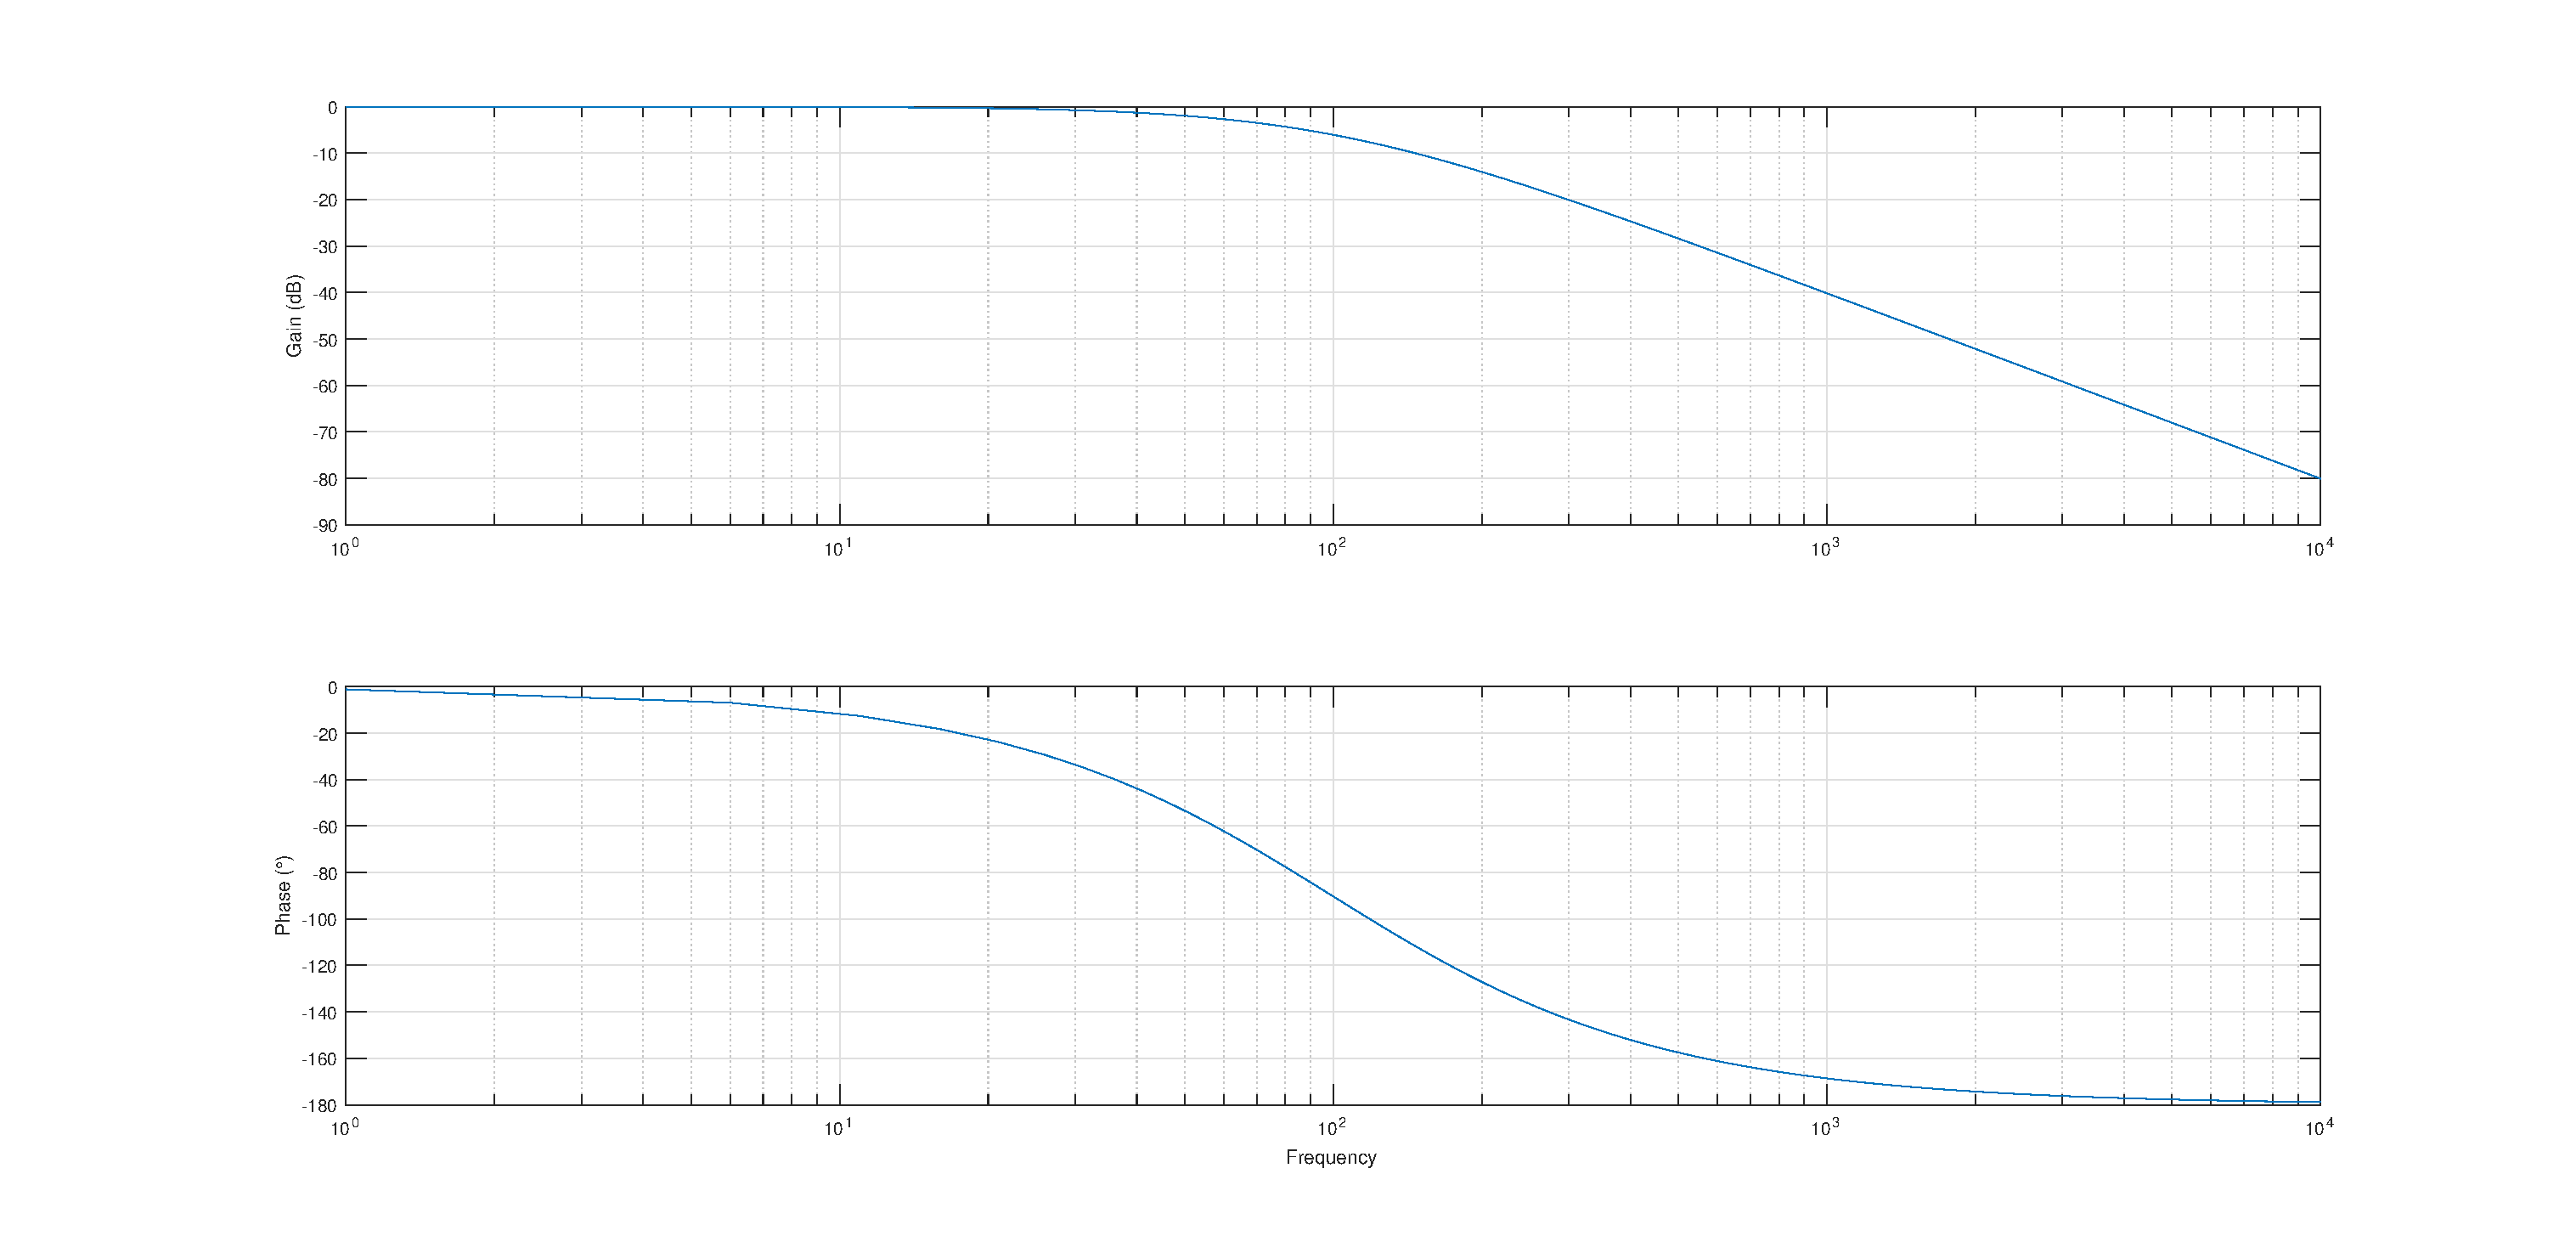
\includegraphics[width=\SchematicWidth]{\Images/Schematic/filter.eps}
    \caption{Bode plot of the filter response}
\end{figure}
\FloatBarrier

The response match our needs, which are quite simple : Remove the potential harmfull noise, 
and fast variations that could occur.

\section{RF Antennas}
For this second section, we're going to explore some RF design steps that we done on the PCB, 
to draw our antennas for the different modules.

This include a $1.55 \si{\giga\hertz}$ for the GPS signals, and a $2.4 \si{\giga\hertz}$ 
Bluetooth antenna.

\subsection{GPS Antenna}

\subsection{Bluetooth Antenna}
For this antenna, we've found a nice application note from TI \cite{InvertedF} that 
show different examples of RF design for 2.4 GHz Antenna. 
Since we don't really know how to properly design an antenna from scratch, we copied this
design into our schematic and PCB.

\section{Power supplies}
Now, let's look a bit deeper on the power supplies, and how they're agenced. 
\subsection{Power tree}
To represent the whole power supply organization, we drew a power tree, a schematic that
represent the power supplies.

% \begin{figure}[!ht]
    \centering
    \resizebox{\SchematicWidth}{!}{%
        \begin{circuitikz}
            \tikzstyle{every node}=[font=\large]
            \draw [ fill={rgb,255:red,195; green,232; blue,235} ] (-1.25,17.25) rectangle  node {\large Battery 1} (3.75,14.75);
            \draw [ fill={rgb,255:red,195; green,232; blue,235} ] (-1.25,11) rectangle  node {\large Battery 2} (3.75,8.5);
            \draw [ fill={rgb,255:red,218; green,187; blue,217} ] (-1.25,4.75) rectangle  node {\large USB} (3.75,2.25);
            \draw [ fill={rgb,255:red,233; green,235; blue,199} ] (8.75,17.25) rectangle  node {\normalsize 5V buck (2A)} (13.75,14.75);
            \draw [ fill={rgb,255:red,233; green,235; blue,199} ] (8.75,11) rectangle  node {\large 3.3V Buck (200 mA)} (13.75,8.5);
            \draw [ fill={rgb,255:red,236; green,195; blue,195} ] (18.75,17.25) rectangle  node {\large Servo and power circuits} (23.75,14.75);
            \draw [ fill={rgb,255:red,158; green,148; blue,213} ] (18.75,11) rectangle  node {\large Logic IC and analog circuits} (23.75,8.5);
            \draw (6.25,4.75) to[D] (6.25,8.5);
            \draw [short] (3.75,3.5) -- (6.25,3.5);
            \draw [short] (6.25,4.75) -- (6.25,3.5);
            \draw [short] (3.75,9.75) -- (8.75,9.75);
            \draw [short] (6.25,8.5) -- (6.25,9.75);
            \draw [short] (3.75,16) -- (8.75,16);
            \draw [short] (13.75,16) -- (18.75,16);
            \draw [short] (13.75,9.75) -- (18.75,9.75);
            \draw [dashed] (6.25,9.75) -- (6.25,16);
            \node [font=\large] at (5,16.5) {7.4V - 8.2V};
            \node [font=\large] at (5,10.25) {4.3V - 8.2V};
            \node [font=\large] at (15.25,16.5) {5V};
            \node [font=\large] at (15.25,10.25) {3.3V};
            \draw [dashed] (6.25,16) -- (6.25,18.5);
            \draw [dashed] (6.25,18.5) -- (16.25,18.5);
            \draw [dashed] (16.25,18.5) -- (16.25,16);
        \end{circuitikz}
    }%
    \label{fig:power_tree}
    \caption{}
\end{figure}
\FloatBarrier TO DO !

On this schematic, there two main regulators, that are, in fact buck switching regulators.
But, there's three power sources : 
\begin{itemize}
    \item   Vbus : The 5V that came from the USBC port when the board is plugged on a PC.
    \item   Vbatt : A battery that is charged to power up the MCU and all of the logic circuits.
    \item   Vbatt\_pyro : A battery that is charged to power up the servo engines and the thruster starter.
\end{itemize}.

We used this kind of architecture to ensure the that the voltage on the control logic remain stable, even when 
a lot of current is drawn on the servo and / or starter, which can easily go above one ampere of current !
In any case, we added some optionnal jumpers to power everything from a single supply, if needed. Theses jumpers
are shown as dotted lines.

\subsection{Microcontroller power supply}

\subsection{Servo power supply}

\section{Digital part}
For the last part, the digital one, we didn't needed a lot of reflexion. Most of the design was already done on 
development kits, for example on the nRF5340DK\cite{nRF5340DK}. Even for sensors, there is mostly the default 
application example that need to be copied, and slightly adapted to our needs.

For example, the modifications we done : 
\begin{itemize}
    \item   Change configuration bootstrap to select one mode of the other.
    \item   Configure power supplies needed.
    \item   Configurd I2C addresses.
\end{itemize}





